\documentclass[12pt]{beamer}
%\documentclass[20pt,handout]{beamer}
\usetheme{Darmstadt}
\usepackage{graphicx}
%\usepackage[german]{babel}
\usepackage[T1]{fontenc}
\usepackage[utf8]{inputenc}
\usepackage{tikz}
\setbeamertemplate{footline}[frame number]

\newcommand{\cc}[1]{\includegraphics[height=4mm]{img/#1.png}}
\usepackage{ifthen}
\newcommand{\license}[2][]{\\#2\ifthenelse{\equal{#1}{}}{}{\\\scriptsize\url{#1}}}
\usepackage{textcomp}

\pgfdeclareimage[height=.6cm]{c3d2logo}{./img/c3d2.pdf} 


\pgfdeclarelayer{foreground}
\pgfsetlayers{main,foreground}
\logo{\pgfputat{\pgfxy(-1,0)}{\pgfbox[center,base]{\pgfuseimage{c3d2logo}}}}


\title{NSA, Prism und co - Wie schützt man sich vor Überwachung?}
\author{\small Marius Melzer \& Stephan Thamm\\\large Chaos Computer Club Dresden}
\date{16.10.2013}

\begin{document}
\maketitle

\section{Einleitung}
\subsection{}

\begin{frame}
  \frametitle{Wer sind wir?}
  \begin{figure}
    
\includegraphics[height=0.7\textheight]{img/fingerabdruck.jpg}
  \end{figure}
\end{frame}

\begin{frame}
  \frametitle{Wer sind wir?}
  \begin{figure}
    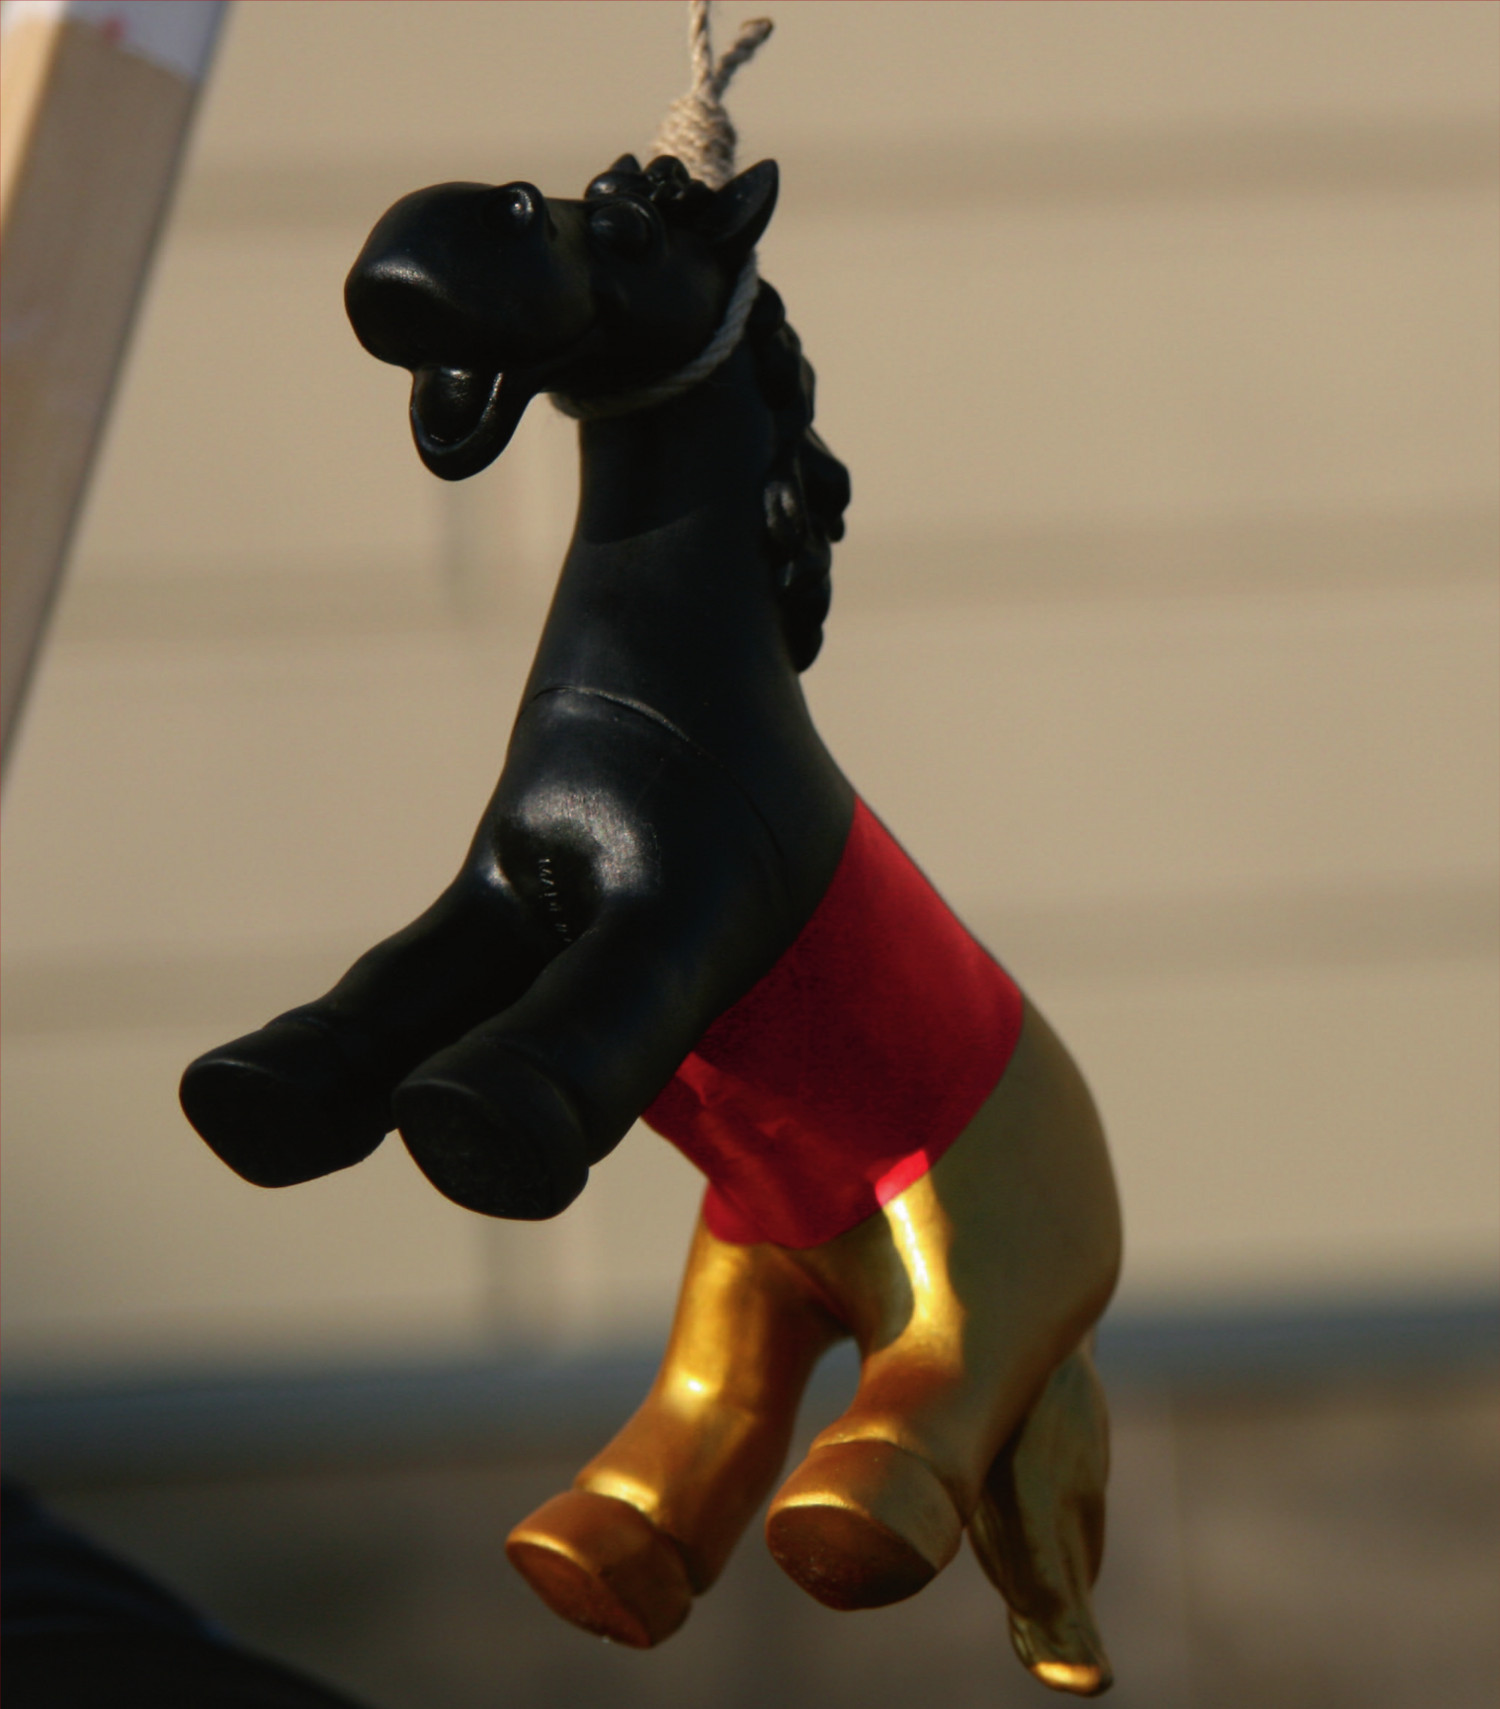
\includegraphics[height=0.7\textheight]{img/trojaner.jpg}
  \end{figure}
\end{frame}

\begin{frame}
    \frametitle{Wer sind wir?}
    \begin{itemize}
      \item<1-> Chaos Computer Club Dresden (\url{http://c3d2.de})
          \note{}
      \item<2-> Datenspuren: Herbst 2014 \url{http://datenspuren.de}
      \item<3-> Podcasts (\url{http://pentamedia.de})
      \item<4-> Chaos macht Schule
    \end{itemize}
\end{frame}

%\ MORE STUFF

\section{Staaten}
\subsection{}

%\ MORE STUFF

\section{Unternehmen}
\subsection{}

\begin{frame}
    \frametitle{Geschäftsmodelle I}
    \begin{itemize}
        \item<2-> Karstadt
        \item<3-> Amazon
        \item<4-> Ebay
        \item<5-> Xing
        \item<6-> Facebook
        \item<6-> Google
    \end{itemize}
\end{frame}

\begin{frame}
    \frametitle{Geschäftsmodelle II}
    \uncover{
        \begin{figure}
            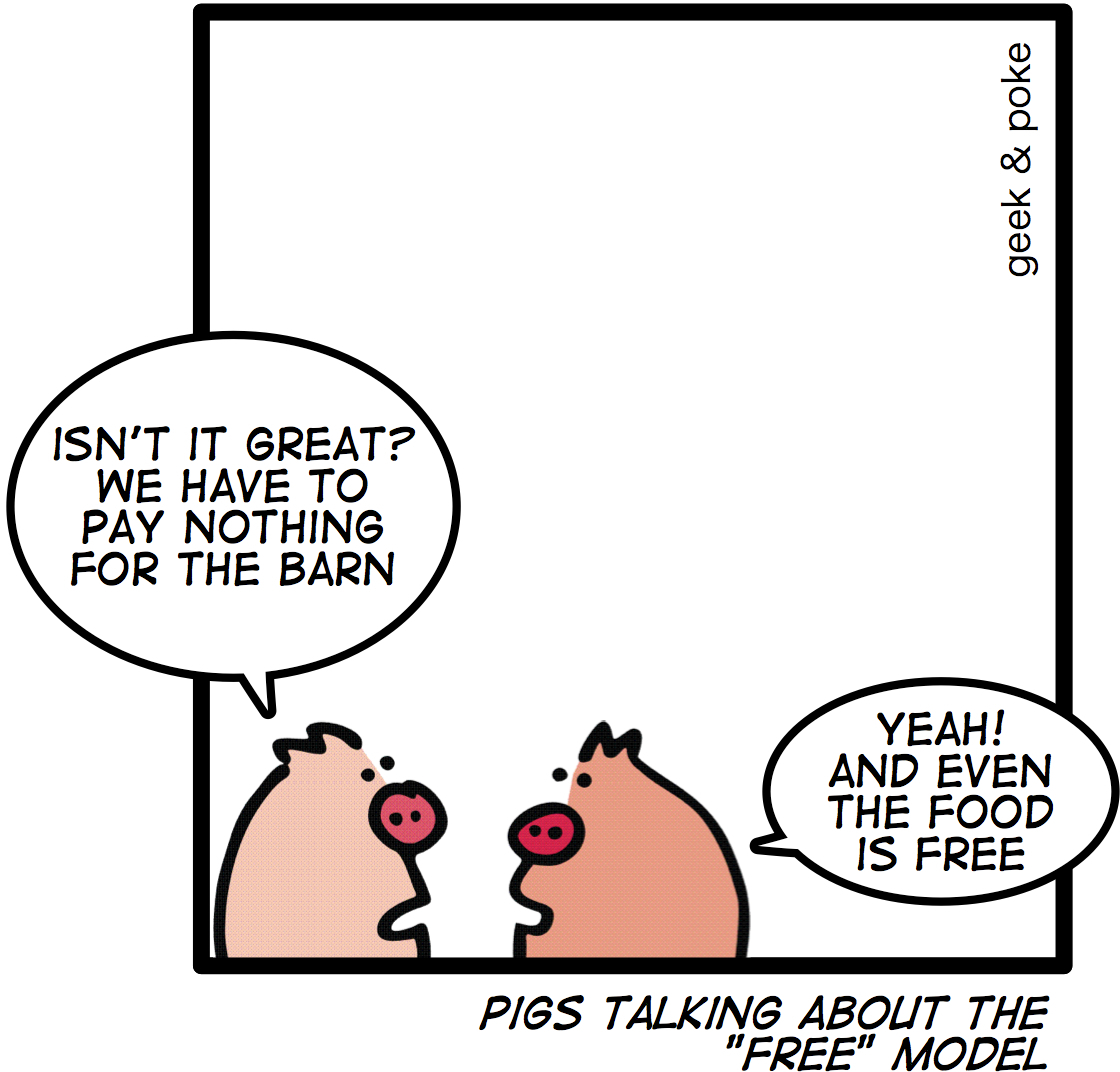
\includegraphics[height=0.6\textheight]{img/business_pigs.jpg}
            \license[http://geekandpoke.typepad.com/geekandpoke/2010/12/the-free-model.html]{\cc{by-sa}}
    \end{figure}}
\end{frame}

\begin{frame}
    \frametitle{Geschäftsmodelle III}
    \begin{center} \Large
        Wofür die ganzen Daten?
    \end{center}
\end{frame}

\begin{frame}
    \frametitle{Datensparsamkeit}
    \begin{itemize}
        \item<2-> Viele Daten zusammen ergeben Profile
        \item<3-> Werden die Daten gebraucht?
        \item<4-> Werden echte Daten gebraucht?
            \begin{itemize}
                \item<5-> Gegenmaßnahme: mailinator.com
            \end{itemize}
    \end{itemize}
\end{frame}

\begin{frame}
    \frametitle{Tracking}
    \begin{itemize}
        \item<2-> Cookies
        \item<3-> Like Buttons
        \item<4-> Werbe- und Statistiknetzwerke
        \item<5-> Gegenmaßnahme: disconnect.me
    \end{itemize}
\end{frame}

\section{Mitmenschen}
\subsection{}

\begin{frame}
    \frametitle{Soziale Netzwerke}
    \begin{itemize}
        \item<2-> Das Internet vergisst nicht!
        \item<3-> Was sollte man (nicht) posten?
            \begin{itemize}
                \item<4-> www.weknowwhatyouredoing.com
            \end{itemize}
        \item<5-> Wer soll den Post (nicht) erhalten?
        \item<6-> Beeinträchtigt der Post andere?
        \item<7-> Gegenmaßnahme: Privatsphäre-Einstellungen
        \item<8-> Gegenmaßnahme: Pseudonymität
    \end{itemize}
\end{frame}

\begin{frame}
    \frametitle{Passwörter}
    \begin{itemize}
        \item<2-> Keine einfachen Wörter
        \item<3-> Groß-, Kleinbuchstaben, Ziffern, Sonderzeichen
        \item<4-> Beispiele:
            \begin{itemize}
                \item<5-> dragon
                \item<6-> (nCuAj.§Tsm!f
                \item<7-> IchLiebeDich
                \item<8-> .§)=")=`
                \item<9-> 123456
                \item<10-> qwerty
                \item<11-> Mks?o/.u,ePsw!
            \end{itemize}
        \item<12-> Verschiedene Passwörter nutzen!
    \end{itemize}
\end{frame}

%\ MORE STUFF

\begin{frame}
    \frametitle{Diskussion}
    \begin{center} {\Large Diskussion}\\Marius Melzer und Stephan Thamm\\CMS Dresden: schule@c3d2.de \end{center}
\end{frame}

\end{document}
